\chapter{\IfLanguageName{dutch}{Stand van zaken}{State of the art}}
\label{ch:stand-van-zaken}

% Tip: Begin elk hoofdstuk met een paragraaf inleiding die beschrijft hoe
% dit hoofdstuk past binnen het geheel van de bachelorproef. Geef in het
% bijzonder aan wat de link is met het vorige en volgende hoofdstuk.

% Pas na deze inleidende paragraaf komt de eerste sectiehoofding.

%Dit hoofdstuk bevat je literatuurstudie. De inhoud gaat verder op de inleiding, maar zal het onderwerp van de bachelorproef *diepgaand* uitspitten. De bedoeling is dat de lezer na lezing van dit hoofdstuk helemaal op de hoogte is van de huidige stand van zaken (state-of-the-art) in het onderzoeksdomein. Iemand die niet vertrouwd is met het onderwerp, weet nu voldoende om de rest van het verhaal te kunnen volgen, zonder dat die er nog andere informatie moet over opzoeken \autocite{Pollefliet2011}.

%Je verwijst bij elke bewering die je doet, vakterm die je introduceert, enz. naar je bronnen. In \LaTeX{} kan dat met het commando \texttt{$\backslash${textcite\{\}}} of \texttt{$\backslash${autocite\{\}}}. Als argument van het commando geef je de ``sleutel'' van een ``record'' in een bibliografische databank in het Bib\LaTeX{}-formaat (een tekstbestand). Als je expliciet naar de auteur verwijst in de zin, gebruik je \texttt{$\backslash${}textcite\{\}}.
%Soms wil je de auteur niet expliciet vernoemen, dan gebruik je \texttt{$\backslash${}autocite\{\}}. In de volgende paragraaf een voorbeeld van elk.

%\textcite{Knuth1998} schreef een van de standaardwerken over sorteer- en zoekalgoritmen. Experten zijn het erover eens dat cloud computing een interessante opportuniteit vormen, zowel voor gebruikers als voor dienstverleners op vlak van informatietechnologie~\autocite{Creeger2009}.

% Te beschrijven in de stand van zaken
% Containers: Hoe werken ze en hoe worden ze gebruikt
% Docker: wat is het en waarvoor wordt het gebruikt?
% Container orkestratie: wat is het en waarom is het nodig
% Kubernetes: wat is het en waarvoor wordt het gebruikt?
% Security: veel voorkomende problemen, best practices
% Security tools: Welke zijn er en hoe werken ze
De stand van zaken of \textit{State of the art} geeft een algemeen beeld weer van de technologieën die worden overwogen in dit onderzoek en tevens de verschillend manieren van toepassing.

\section{Containers} \label{containers}
In dit hoofdstuk zal uitgelegd worden wat containers zijn, hoe ze werken en waarvoor ze worden gebruikt.

Containers bieden veel voordelen vergeleken met normale virtuele machines (VM's). Ze kunnen snel opgezet worden en zijn gemakkelijk om te configureren terwijl virtuele machines vaak groot en traag zijn. Containers zijn pakketten waarin een applicatie vervat zit, samen met zijn benodigde bibliotheken en afhankelijkheden. Hierdoor kunnen ze vlot van de ene omgeving naar de andere worden overgezet zonder dat er extra configuratie nodig is \autocite{Education2019}. Containers maken gebruik van besturingssysteem-virtualisatie om processen te isoleren van het \textit{host} besturingssysteem. Daarnaast controleert het tevens de CPU gebruik en hoeveelheid RAM geheugen van deze processen (Docker, 2018).

Containers hebben eigenlijk geen eigen besturingssysteem nodig, alle containers delen 1 gezamenlijke \textit{runtime engine}. Een \textit{runtime engine} is de laag die verantwoordelijk is voor de communicatie tussen het besturingssysteem van de host machine en de containers zelf. De meeste gebruikte runtime engine is de \textit{Docker Engine}\footnote{docs.docker.com/engine/}.

\subsection{Container vs. virtuele machine}
\subsubsection{Hypervisors}
Bij traditionele virtuele machines virtualiseert een \textit{hypervisor} de fysieke hardware. De hypervisor regelt het resource gebruik tussen de verschillende VM's en zorgt ervoor dat de hardware van de host (de fysieke hardware waar de hypervisor op geïnstalleerd is) eerlijk verdeelt wordt. Er zijn 2 types hypervisor \autocite{VMWare2021}, namelijk:
\begin{itemize}
    \item Type 1: Ook wel \textit{bare metal} hypervisors genoemd. Deze werken rechtstreeks op de fysieke hardware van de host en hebben dus geen onderliggend besturingssysteem nodig. Door het rechtstreekse contact tussen de hypervisor en de hardware wordt een type 1 hypervisor beschouwd als de best presterende en meest efficiënte hypervisor. Een type 1 hypervisor wordt ook beschouwd als het veiligste van de 2, dit omdat de gebreken en kwetsbaarheden die doorgaans in besturingssystemen aanwezig zijn hier onmogelijk zijn.
    \item Type 2: Ook wel \textit{hosted} hypervisors genoemd. Deze worden doorgaans geïnstalleerd op een bestaand besturingssysteem en steunt daar ook op voor het beheren van de resources. Een groot voordeel van type 2 hypervisors is dat ze een breed gamma aan hardware ondersteunen.
\end{itemize}
\begin{figure}[ht]
    \centering
    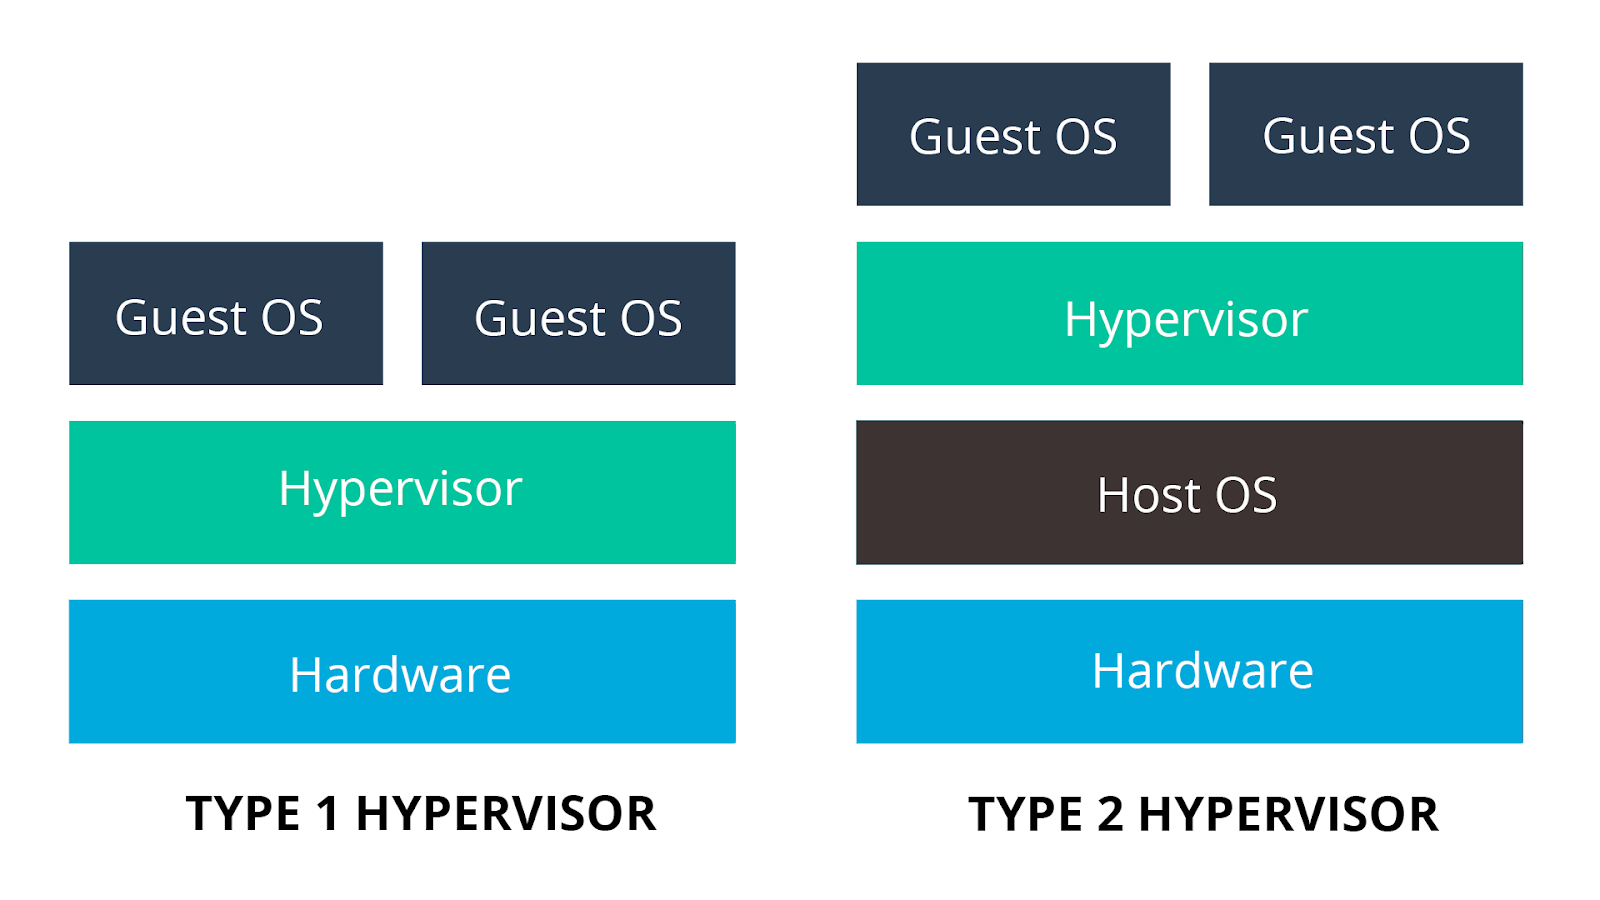
\includegraphics[width=\linewidth]{img/Hypervisor.png}
    \caption{Type 1 \& Type 2 Hypervisor \autocite{VMWare2021}}
    \label{fig:hypers}
\end{figure}

Tegenwoordig worden type 1 hypervisors in productieomgevingen het meest gebruikt, dit vanwege hun efficiënte resource gebruik en veiligheid. Type 2 hypervisors worden meer gebruikt in testomgevingen omdat deze gemakkelijker op zetten zijn.

Elke Vm heeft zijn eigen volwaardg besturingssystemen, met gevolg dat deze veel resources gebruiken en hierbij vaak trager zijn. In plaats van de onderliggende hardware te visualiseren gebruiken containers het besturingssysteem (meestal is dit Linux) zelf, zo bevat elke individuele container enkel de applicatie en de bijhorende bibliotheken en afhankelijkheden bevat \autocite{Education2020}.

\begin{figure}[ht]
    \centering
    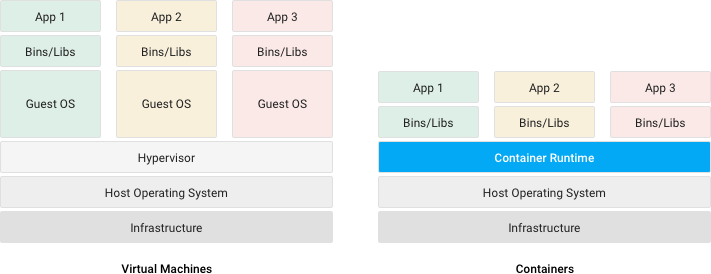
\includegraphics[width=\linewidth]{img/container-vs-vm.png}
    \caption{Container vs. virtuele machine \autocite{Google2016}}
    \label{fig:example}
\end{figure}


\subsection{Waarvoor worden containers gebruikt}
Containers zijn zeer veelzijdig en kunnen dus in veel verschillende omstandigheden gebruikt worden. Enkele \textit{use cases} waarvoor containers zeer geschikt zijn \autocite{Docker2021}:

\begin{itemize}
  \item \underline{Microservices}: Containers zijn klein en licht, waardoor ze goed passen bij microservice-architecturen waarin applicaties zijn opgebouwd uit vele, losjes gekoppelde en onafhankelijk services.
  \item \underline{Modernisering en migratie van applicaties}: Een van de meest voorkomende benaderingen voor het moderniseren van applicaties begint met het containeriseren ervan, zodat ze naar de \textit{cloud} kunnen worden gemigreerd.
  \item \underline{Nieuwe ontwikkelaars snel inwerken}: Door gebruik te maken van containers verloopt het opzetten van een nieuwe lokale ontwikkelingsomgeving snel en vlot, hierdoor kunnen de ontwikkelaars direct aan de slag.
\end{itemize}


\section{Docker}
\textit{Docker}\footnote{docker.com/} is een open source container platform dat sinds de release in 2013 ongelofelijk populair is geworden. In november 2019 stond de teller van aantal \textit{pulls} op de \textit{Docker hub} op 130 miljard, in juli 2020 stond deze al op 242 miljard. Dat is bijna dubbel op minder dan 8 maand tijd \autocite{Kreisa2020}. Docker-containers kunnen overal draaien, in het datacenter, bij een externe serviceprovider of in de cloud. Docker containers kunnen zowel op Linux als op Windows draaien. Containers die op Windows gebaseerd zijn kunnen echter alleen op Windows systemen draaien, maar Linux containers kunnen op zowel Linux systemen en Windows systemen draaien (met behulp van een Linux VM). Dit komt omdat containers ontworpen zijn om het besturingssysteem van de host te gebruiken \autocite{Anil2018}.


\subsection{Hoe werkt docker}
Docker gebruikt een \textit{Client-Server} architectuur. Deze werkt als volgt: De Docker \textit{Client} communiceert met de Docker \textit{Deamon} (een proces dat op de achtergrond draait en bepaalde (onderhouds-)taken uitvoert). Deze is verantwoordelijk voor het bouwen, runnen en verspreiden van containers \autocite{Docker2021a}.

\subsection{Docker componenten en terminologie}

\subsubsection{Docker Deamon}De Docker Daemon (\verb|dockerd|) luistert naar Docker Application programming interface (API) verzoeken en beheert Docker objecten waaronder \textit{images}, \textit{containers}, netwerken, en \textit{volumes}.

\subsubsection{Docker Client}De Docker Client is de meest gebruikte manier voor gebruikers om te communiceren met Docker. De client stuurt alle ingevoerde commando's (zoals \verb|docker pull| en \verb|docker run|) door naar de Docker Daemon die deze uitvoert.

\subsubsection{Docker registries}
Een \textit{Docker register} is een bibliotheek die \textit{Docker images} opslaat. Het standaard register voor Docker is de \textit{Docker Hub}\footnote{hub.docker.com/}. Als de Docker daemon geen lokale Docker image vindt gaat deze standaard in de \textit{Docker Hub} zoeken. Wanneer gebruik gemaakt wordt van de \verb|docker pull| of \verb|docker run| commando's wordt gebruikt, worden de benodigde images uit het register gehaald.

\subsubsection{Docker objecten} \label{dockerObjects}
Docker maakt gebruik van images, volumes en netwerken, al deze onderdelen worden objecten genoemt. Volgens \textcite{Docker2021a} zijn dit de belangrijkste objecten:

\begin{itemize}
        \item \textbf{Images}: Docker images zijn \textit{read-only} sjablonen met instructies om een Docker container op te zetten. Docker images kunnen uit de Docker hub gehaald worden en direct gebruikt worden zonder verdere configuratie. Verder kan je tevens bijkomende instructies toevoegen aan de \textit{base image} en deze opslaan als een nieuwe en aangepaste Docker image. Een Docker image is vaak gebaseerd op een andere images (i.e., Een nieuwe image kan gebaseerd zijn op een bestaande \textit{Ubuntu} image maar installeert en configureert daarbij een \textit{Apache} webserver). Alsook is het mogelijk om zelf een compleet nieuwe image te maken met behulp van een \textit{dockerfile}.
        \item \textbf{Containers}: Een container is een uitvoerbare instantie van een image die wordt gecontroleerd via de Docker API. Een container kan verbonden worden met andere containers, aan externe opslag of gebruikt worden als basis voor nieuwe image.
        \item \textbf{Volumes}: De persistente gegevens die Docker containers kunnen gebruiken wordt opgeslagen in zogenaamde volumes. Deze volumes worden volledig gecontroleerd via de Docker API en bevinden zich buiten de container zelf. Hierdoor blijft het gewicht van de containers laag en kan de data blijven bestaan ook al wordt de container gestopt of verwijderd.
\end{itemize}

\section{Container orkestratie}
Container orkestratie helpt bij het opzetten, beheren, schalen en verbinden van een grote hoeveelheid containers. Container orkestratie helpt dus om complexe procedures te vergemakkelijken. Dit door veelvoorkomende processen en werkstromen te stroomlijnen en te optimaliseren. Een ander belangrijk onderdeel van orkestratie is het geautomatiseerd onderhoud van de applicaties die in de containers draaien \autocite{RedHat2021}.

\subsubsection{Waarvoor word container orkestratie gebruikt?}

Container orkestratie wordt vooral gebruikt voor het automatiseren en beheren van de configuratie en uitrol, het toewijzen van resources, de \textit{Load balancing} en het monitoren van containers.
%Container orkestratie wordt vooral gebruikt voor het automatiseren en beheren van:
%\begin{itemize}
%    \item De configuratie en uitrol van containers.
%    \item De toewijzing van resources.
%    \item De \textit{Load balancing} op basis van de belasting van het systeem.
%    \item Het monitoren van containers.
%    \item De beveiliging van interacties tussen containers.
%\end{itemize}

\subsection{Container orkestratie tools}
Om aan container orkestratie te gaan doen zijn er natuurlijk tools nodig die ons alle nodig functionaliteiten kunnen aanbieden. \textcite{DevopsCube2021} geeft een overzicht van de meest prominente orkestratie tools.

\subsubsection{Kubernetes}
Kubernetes(K8s)\footnote{kubernetes.io/} is een open-source, container cluster manager en orchestratie tool. Het is gebouwd met een uitstekende resource manager voor het inzetten van containers op een efficiëntere manier. Kubernetes is voor vele organisaties de ``de facto'' container orkestratie tool geworden voor veel organisaties. Volgens \textcite{CNCF2021} zijn er meer dan 109 tools om containers te beheren, maar 89\% is gebouwd met K8s aan de basis.

\subsubsection{Openshift}
Openshift behoort tot de 89\% tools die gebouwd zijn bovenop Kubernetes. Het Openshift-project\footnote{openshift.com/} word onderhouden door RedHat\footnote{redhat.com/}. Het heeft zowel een open source versie (\textit{openshift origin}\footnote{github.com/openshift/origin}) als een enterprise versie (\textit{openshift container platform}\footnote{openshift.com/products/container-platform}).

\subsubsection{Hasicorp Nomad}
Nomad\footnote{nomadproject.io/} is een orkestratieplatform van Hashicorp\footnote{hashicorp.com/} dat containers op schaal kan ondersteunen. Op het vlak van applicatiemanagement is het zeer sterk vergelijkbaar met Kubernetes. Echter kan Nomad ook niet-containerapplicaties kan beheren, met gevolg dat deze zich kan distantiëren van de andere orkestratie tools. Daarnaast kan Nomad feilloos geïntegreerd worden met andere tools van Hashicorp.

\section{Kubernetes}
Hier wordt ingegaan op wat Kubernetes(K8s)  en hoe het werkt. Daarnaast worden de verschillende technische termen die eigen zijn aan K8s uitgelegd.

Kubernetes is een open-source, container cluster manager en orchestratie tool. Het werd ontwikkeld door Google om hun container applicaties op grote schaal te kunnen orkestreren. Het project werd in 2014 \textit{open-source} gemaakt, dat wil zeggen dat Google niet meer rechtstreeks de eigenaar is maar dat het project verder ontwikkeld wordt door vrijwilligers. Hierdoor konden ook andere organisaties niet alleen gebruik maken van deze krachtige tool, maar tevens meewerken aan de ontwikkeling ervan. De term \textit{Kubernetes} is Grieks voor 'stuurman van een schip' \autocite{Kubernetes2021}. Enkele diensten die door K8s aangeboden worden:
\begin{itemize}
    \item Automatisch load-balancing op basis van de hoeveelheid verkeer.
    \item Opslag orkestratie: Het automatisch \textit{mounten} van verschillende types opslag (lokale- of cloud opslag).
    \item Resource controle: K8s zorgt ervoor dat de beschikbare resources correct en efficiënt verdeeld worden.
    \item \textit{Self-healing}: K8s kan containers heropstarten, vervangen of stopzetten als deze niet meer voldoende correct werken.
\end{itemize}
\textbf{\textit{Mogelijks is volzinnen uitschrijven!!!!}}

\subsubsection{Kubernetes componenten en terminologie}
Zoals beschreven in de documentatie van \textcite{Pedersen2021, RedHat2021a} worden Kubernetes en de bijhorende componenten als volgt gedefinieerd: Kubernetes is een \textit{cluster} bestaande uit 2 grote delen namelijk het \textit{control plane} en de \textit{nodes}. Deze nodes zijn de door K8s georkestreerde containers. Elke cluster bestaat uit uit minstens één, maar meestal meerdere, nodes. De nodes worden gebruikt om \textit{pods} te hosten. Pods zijn de kleinst mogelijke eenheid in een K8s systeem. Een pod bestaat uit één of meerdere containers die opslag- en netwerk resources delen \autocite{RedHat2021a}. In Figuur \ref{fig:K8sComponents} worden de verschillende componenten van een K8s cluster gevisualiseerd.

\begin{figure}[ht]
    \centering
    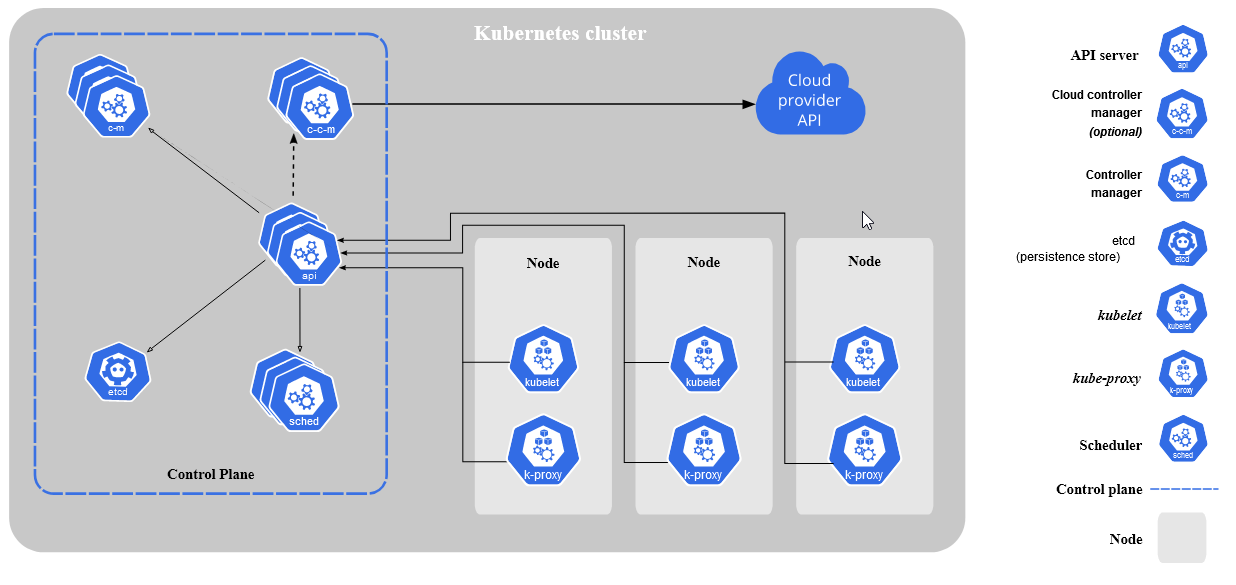
\includegraphics[width=\linewidth]{img/kubernetes-components.png}
    \caption{Kubernetes cluster componenten \autocite{Kubernetes2021}}
    \label{fig:K8sComponents}
\end{figure}

Het hart van een K8s cluster is de \textbf{\textit{Control plane}}, hierin bevinden zich alle componenten die de cluster controleren.Tevens zitten alle gegevens omtrent de staat van de cluster en de configuratie hierin verbonden. Alle componenten die deel uitmaken van de \textit{Control plane} kunnen op verschillende machines draaien. ierbij wordt aangeraden om wordt aangeraden om deze binnen eenzelfde machine te houden. De verschillende onderdelen en hun plaats binnen een cluster worden hieronder besproken.

De \textbf{\textit{kube-apiserver}} wordt gezien als de \textit{Front-end} van een Kubernetes cluster. Deze is de link tussen \textit{nodes} en \textit{pods} van de cluster en de \textit{Control plane}. Het doel van deze apiserver is om de communicatie van de nodes en de Kubernetes API to bolwerken. De apiserver is ontworpen om horizontaal te schalen als deze te zwaar belast wordt. Hierbij creëert hij nieuwe instanties van zichzelf.

Alle data en informatie met betrekking tot de status van de cluser wordt opgeslagen in \textbf{\textit{etcd}}, een \textit{key-value store database}.

De \textbf{\textit{kube-scheduler}} is verantwoordelijk voor het toekennen van pods aan nodes en voor het verdelen van de resources tussen de verschillende Nodes. Het toekennen van een Node aan een Pod gebeurdt aan de hand van verschillende factoren. De mogelijke factoren zijn onder andere de benodigde resources van een Pod en eventuele harware- en sofware beperkingen.

Een \textbf{\textit{kube-controller-manager}} bestaat uit verschillende \textit{controllers} die allemaal een verschillende taak op zich nemen. Enkele van deze \textins{controllers} zijn:
\begin{itemize}
    \item \textit{Node controller}: Het hoofddoel van deze controller is om op te merken en reageren als er Pods zouden wegvallen.
    \item \textit{Job controller}: Deze zoekt naar zogenaamde \textit{job-objecten}, die eenmalige taken voorstellen, en creëert bijgevolg de nodige Pods om deze taken uit te voeren.
    \item \textit{Service Account \& Token controllers}: Deze creëert standaard accounts en \textit{API access tokens} voor nieuwe Pods.
\end{itemize}

Als het \textit{Control plane} het hart van een K8s cluster is dan kunnen we de \textit{Nodes} het lichaam noemen. Deze doen namelijk al het zware werk en worden bestuurd door de \textit{Control plane}.

Het eerste onderdeel van een Node is de \textbf{\textit{kubelet}}, een kleine applicatie die op elke Node aanwezig is. De \textit{kubelet} houdt de gezondheid en status van de Pods, die binnen zijn Node draaien, in het oog. Wanneer de \textit{Control plane} wil dat er iets gebeurd met de Node zorgt de \textit{kubelet} ervoor dat deze acties correct uitgevoerdt worden.

De \textbf{\textit{kube-proxy}} is een netwerk \textit{proxy} die de verantwoordelijk is voor de K8s \textit{networkservices}. De \textit{kube-proxy} verzorgt netwerkcommunicatie zowel binnen- als buiten de cluster.

Het volgende component, namelijk de \textbf{\textit{Container runtime}}, werd al reeds besproken in sectie \ref{containers}.

Ten slotte zijn er nog enkele extra \textit{addons} die gebruikt kunnen worden om de functionaliteit van een K8s cluster uit te breiden. Een eerste voorbeeld van een \textit{addon} is de mogelijkheid om persistent geheugen (ook wel \textit{volumes} genoemd) toe te voegen zoals uitgelegd in sectie \ref{dockerObjects}. Andere voorbeelden zijn het toevoegen van een \textbf{\textit{cluster DNS}}, \textbf{\textit{Web UI}} of \textbf{\textit{Dashboard}} en het opslaan van de log bestanden van de cluster met \textbf{\textit{cluster-level logging}}.

\section{Security}
Hier word het security aspect van containers en container orkestratie besproken. (redelijk high level want kan ongelooflijk complex worden)


Uit een raport van \autocite{Tripwire2019} blijkt dat 94\% van bevraagden bezorgd zijn over de veiligheid van hun containers. Uit hetzelfde rapport blijkt ook dat 47\% weet dat ze mogelijks kwetsbare containers gebruiken in hun productieomgeving.

ALGEMENE SECURITY ZEVER (beetje me nummers smijten/CVE bespreken?)


\subsection{Meest voorkomende security problemen}
Hier worden de meest voorkomende security problemen opgelijst en worden ze kort besproken (Technische uitleg over hoe deze problemen onstaan)

Uitleg over hoe k8s security eruit ziet + wat voor exploits daarmee onmogeleijk gemaakt worden

\subsection{Hoe een container cluster beveiligen}
Uitleg over hoe een container cluster beveiligt kan worden

- ingebouwde security features
    - CNI's
- Best practices

\section{Security tools}
Hier worden enkele security tools opgeslijst en hun werking kort besproken.

Een andere manier om een K8s cluster te verder te beveiligen is door gebruik te maken man verschillende \textit{Security tools}.
 \textcite{Taylor2019} geeft een overzicht met de mest prominente tools. Deze zullen hieronder besproken worden.

\subsection{Project Calico}

\textbf{\textit{Project Calico}}\footnote{projectcalico.org/} is volledig \textit{open source} en volgens \textcite{Armstrong2021} de meeste gebruikte security tool voor K8s. Calico is niet enkel een K8s security tool maar is ook volledig geïntegreerd met vele andere platformen. Figuur \ref{fig:CalicaEco} geeft een overzicht van de door Calico ondersteunde platformen. Project Calico creert een soort van \textit{microfirewall} rond elke service. De policies die ingesteld kunnen worden in Calico worden automatisch omgezet naar firewall regels. Deze worden vervolgens toegepast op elke service. Calico heeft zich onlangs aangesloten bij de Cloud Native Computing Foundation(CNCF), waardoor het onder deskundig toezicht staat en nog beter geïntegreerd is in het Kubernetes ecosysteem.
\begin{figure}[ht]
    \centering
    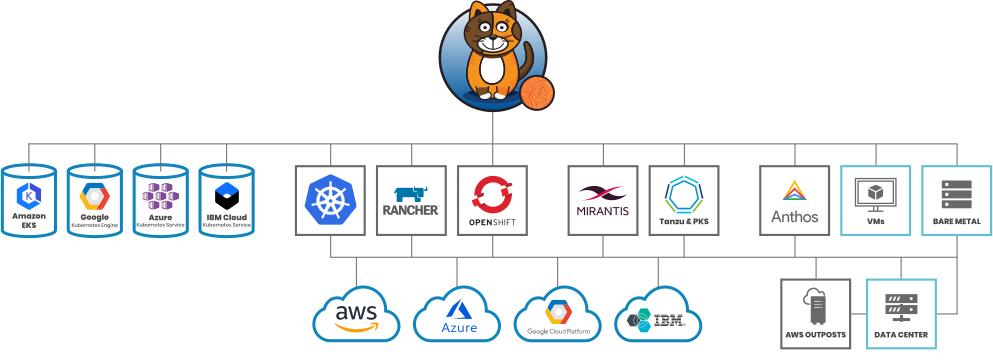
\includegraphics[width=\linewidth]{img/Calico-Ecosystem.png}
    \caption{Platformen die ondersteunt zorden door Calico \autocite{Tigera2021}}
    \label{fig:CalicaEco}
\end{figure}

\subsection{Kube-Bench}
\textbf{\textit{Kube-Bench}}\footnote{github.com/aquasecurity/kube-bench} is een \textit{open-source} applicatie geschreven in \textit{Go}\footnote{golang.org/} die controleert of k8s veilig is geïmplementeerd door controles uit te voeren op de cluster. De controles zijn gebaseerd op enkele guidelines die het \textit{Center for Internet Security}\footnote{cisecurity.org/benchmark/kubernetes/} (CIS), een organisatie die richtlijnen opmaakt voor het schrijven van veilige code, heeft opgesteld. Het is verpakt als een container en kan dus zeer snel en gemakkelijk in gebruik genomen worden. \textit{Kube-Bench} controleert niet alleen of er fouten in de beveiliging van een cluster zitten, het geeft ook mogelijke oplossingen. Enkele van de controles die gebeuren zijn het controleren van gebruikersautorisatie en -authenticatie, de versleuteling van gegevens en kijken of de cluster het principe van \textit{least privilege} volgt (een gebruiker krijgt enkel toegang tot gegevens die hij echt nodig heeft). De testen worden gedefinieert een in `YAML Ain't Markup Language' (YAML) bestand zodat ze gemakkelijk aangepast en uitgebreid kunnen worden \autocite{Rice2021}. De test worden uitgevoerd op elke individuele node in de cluster waardoor het vooral geschikt is voor kleinere opstellingen.

\subsection{Kube-hunter}

\textbf{\textit{Kube-hunter}}\footnote{github.com/aquasecurity/kube-hunter} is, net zoals \textit{Kube-Bench}, een open-source applicatie gemaakt is door \textit{Aqua Security}\footnote{aquasec.com/}. \textit{Kube-hunter} breidt de functionaliteiten van \textit{Kube-Bench} uit door penetratie testen uit te voeren op de cluster. Dit zorgt ervoor dat administrators problemen met een cluster gemakkelijk kunnen opsporen en verhelpen.